\chapter[Neutral MSSM Higgs Bosons Search...]{Search for neutral MSSM Higgs Bosons in the 
$A/h/H \rightarrow \tau^{+}\tau^{-} \rightarrow e \mu + 4\nu$ decays} \label{chap:anal}

%A search for neutral MSSM Higgs bosons with the ATLAS detector at the
%LHC is presented.  This analysis is based on an integrated luminosity of $20.3 ~fb^{-1}$
%of proton-proton collisions at a center-of-mass energy of 8 TeV. 
%
%The analysis focusses on the decay of neutral Higgs bosons into a pair of tau
%leptons, which subsequently decay to an electron, a muon and four
%neutrinos. Furthermore, 
%
Under the light of the recent discovery of a Higgs 
boson with mass of 125 GeV \cite{}, remains an open question
wheter this new particle constitute all the pieces of the Higgs
sector or wheter it is only one of several bosons predicted in some theories 
that go beyond the SM. The most recent measurements \cite{} of its
properties shows it to be, within experimental uncertainties, perfectly 
compatible with the SM Higgs boson, however such a new particle can 
be accomodated within several beyond the 
standard model (BSM) theories, this is particularly true for Super Symmetry. 

There are two approach to explore the Higgs sector:
one can study the cupling of the Higgs boson with vector
bosons and fermions, those measure in fact are sensitive to new physics and can determine
%given the unitarity property of scattering
%aplitudes for longitudinal vectors and fermions, one can understand 
if this particle is  fully responsible for
the generation of all the SM particles masses. 
Another approach is to directly search for %model dependent
for additional Higgses in a well defined model, which is the approach followed in this
thesis where new neutral bosons are sought within the MSSM (see chapter \ref{}). 


%Discovering the mechanism responsible for electroweak
%symmetry-breaking and the origin of mass for elementary particles has been
%one of the major goals of the physics program at the Large Hadron
%Collider~(LHC)~\cite{LHC}.  In the Standard Model (SM) this mechanism
%requires the existence of a single scalar particle, the Higgs
%boson~\cite{ENGLERT,HIGGS,HIGGS2,HIGGS3,Guralnik:1964eu}.

%This chapter is divided in three sections:
%in section~\ref{sec:strategy} an introduction to experimental searches and to the strategy
%of this particular analysis is given, in section~\ref{sec:bkg} is described the core of this thesis
%work, i.e. the detail of the background modeling for this analysis, while in section~\ref{sec:result}
%the result of the sarch are presented.


\clearpage

%%\section{Inside Neutral MSSM Higgs}
%\section{What is a Search?}
%\section{Search First Principle}
%\section{Search Elements}
%\section{The Search in a Nutshel}
\section{Introduction}
\label{sec:strategy}

%\subsection{Motivation}

\begin{figure}[tp]
     \begin{center}

            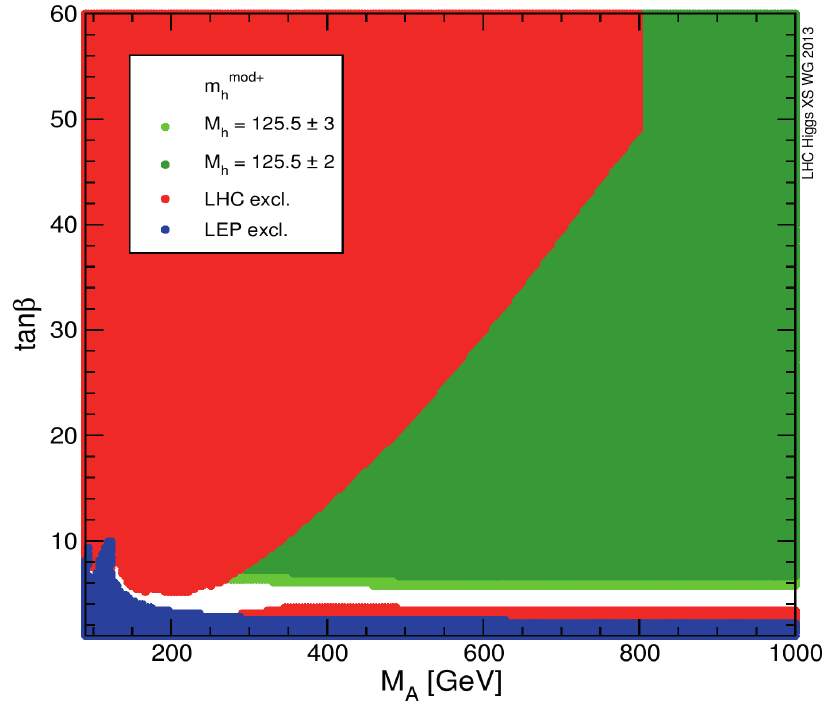
\includegraphics[width=0.6\textwidth]{figure/mh_mod.png}

    \end{center}
    \caption{Excluded and allowed regions of the $m_{A} - \text{tan}\beta$ parameter space for the  $m_{h}^{mod+}$ 
	benchmark scenario. Excluded region are determined based on direct Higgs boson searches at LEP (blue) and LHC (red). The two green 
	bands corresponds to the parameter regions which are compatible with the assumption that 
	the lightest Higgs boson, \emph{h}, has a mass respectively of $M_{h} = 125.5 \pm 2$ or $\pm 3$ GeV. For more detail 
	see~\cite{LHCxsec}.}
   \label{fig:mhmod}
\end{figure}

In the Minimal Supersymmetric extension of the Standard Model
(MSSM)~\cite{MSSM1, MSSM2} the Higgs sector is composed of two Higgs
doublets of opposite hyper-charge, resulting in five observable Higgs
bosons.  Two of these Higgs bosons are neutral and $CP$-even
($h$,$H$), one is neutral and $CP$-odd ($A$) and two are charged
($H^\pm$).  At tree level their properties such as masses, widths and
branching ratios can be predicted in terms of only two parameters,
often chosen to be the mass of the $CP$-odd Higgs boson $m_A$, and
the ratio of the vacuum expectation values of the two Higgs doublets
$\tan\beta$ (for more details see chapter~\ref{chap:theory}).  

The MSSM predicts the existence of a Higgs boson with properties that  
resemble those of a SM Higgs boson in large regions of its parameter space. It is technically impossible,
for an experimental  search, to explore the full parameter space of the model, several benchmark scenarios are then 
introduced by fixing the parameters to values typical for most interesting physics scenarios.
% a point in the MSSM parameter space must now not only pass all the 
%experimental bounds on superparticle masses, but also lead to the prediction of a scalar with
%mass, production cross section and decay rates compatible with those measured at the LHC.
%it is not convenient to scan over a large parameter space as the MSSM has, for practical reason
With the recent Higgs boson discovery, bechmark scenarios of the MSSM have been updated to 
accomodate for  new experimental constraints (see chapter~\ref{chap:theory}). 
As an example, Figure~\ref{fig:mhmod} shows the currently excluded and allowed regions of the MSSM parameter space
for the  $m_{h}^{mod+}$ updated benchmark scenario. In this scenario a supersymmetric SM-like Higgs boson is assumed, 
large region of the $m_{A} - \text{tan}\beta$ parameter space is compatible with this assumption and remains still unexplored.


This chapter presents the search for the neutral MSSM Higgs bosons decaying into pairs of tau leptons
in the fully leptonic final state. The search is based on 20.3 $\text{fb}^{-1}$ of 8 TeV data 
recorded by the ATLAS experiment during 2012 at the Large Hadron Collider~(LHC)~\cite{LHC}.
Higgs boson candidated events are selected based on the topological properties of the Higgs boson production 
and decay. The two dominant Higgs boson production modes are via gluon-gluon fusion and in association with b-quarks,
the search take advantage of that being performed separately for events without or with b-tagged jets in the final state,
respectively. Two of the dominat background contributions, $\Ztautau$ and multi-jet process, are predicted with 
the corresponding signal-depleted control data samples. The final statistical interpretation of the data is based on the 
comparison of the observed invariant mass distributions, exclusion limits are set by means of a binned likelihood ratio
test statistic and interpreted either in the MSSM $m_{h}^{max}$ scenario and in a model independed.

In the MSSM for large region of parameter space one found that one of the 
$CP$-even neutral Higgses  has properties that resemble the one of the SM Higgs,
this is usually the case for the lightest Higgs, \emph{h}, the other two, $H$ and $A$, 
tend to be degenerate in mass and decouple from gauge bosons.
An interesting fenomenological consequence is that the coupling of the latter
two Higgses with down (up) type fermions are enhanced
(suppressed) by $\tan\beta$, meaning that for large $\tan\beta$
bottom-quark and $\tau$ lepton will play a more important role than in
the SM case either for production and decay.

The production of the neutral $CP$-even MSSM Higgs bosons at hadron
colliders proceeds via the same processes as for the SM Higgs
production. However, the pseudoscalar $A$ instead cannot be produced
in association with gauge bosons or in vector boson fusion (VBF) at
tree-level, as this coupling is forbidden due to $CP$-invariance.  At
the LHC one of the most relevant production mechanisms for the MSSM
Higgs bosons is gluon-gluon fusion, $gg\rightarrow A/H/h$. In
addition, the production in association with $b$-quarks becomes
important for large value of $\tan\beta$. Those are the two production mechanism
that are considered in this analysis, Figure~\ref{fig:prod} shows the Feynman-diagram
for those processes, while Figure~\ref{fig:xsec} shows the production cross section of the neutral 
MSSM Higgses via these two processes. The search is divided in two category which are optimized
for the two different production mode considered, in the gluon-fusion category
is requred a b-jet veto (for definition of b-tagging algorithm see chapter~\ref{chap:detector}), in fact no b-jet in the final state are present for this
production mode. In contrast a a b-jet tag is required for b-associated production,
this category is expected to be very sensitive to $\tan\beta$. The two category are
ortogonal and present different backgrounds contributions, which can be
optimized separately. 

The decays of the neutral
MSSM Higgs bosons (in the assumption that all supersymmetric particle
are heavy enough) are the same as for the SM one with the already
cited exception of $A$. Figure~\ref{fig:xsec} shows the decay branching fractions
for $H$ and $A$ as a function of the mass, 
the decay into tau pair is the most important after $b\bar{b}$ and the one used in this analysis. The 
decay channel in $b\bar{b}$ is in fact very challenging due to the huge background from
QCD multi-jet.
In this thesis only cases in which the taus decay one in $e + 2\nu$ and
the other in $\mu + 2\nu$ are considered, This final state corresponds to a total
$\tau^+\tau^-$ branching ratio of approximately 6\%.
 
The signal topology described in the previous section is common to many other processes, unfortunately, 
those have higher cross section than the sought signal and a set of additional selections
is needed to enhance the sensitivity of the search.
The most important backgrounds to this search are the production of
 $\Ztautau $ + jets, the top quark ($t\bar{t}$ and single top production is intended), diboson production 
(like $WW$ or $ZZ$ events) and Drell-Yan process or events with non-prompt leptons coming 
solely from hadron decay (in short QCD multi-jet).
Vector bosons production like  $\Wlnu$ or $\Zll$ + jets (with $\ell$ here meaning either $e$ or $\mu$) are also considered,
however those processes have a limited impact.

%Searches for neutral MSSM Higgs bosons have been performed at
%LEP~\cite{LEPLimits}, the
%Tevatron~\cite{TevatronLimits1,TevatronLimits2,TevatronLimits3,TevatronLimits4,TevatronLimits5,TevatronLimits6}
%and the LHC~\cite{CMSLimit, ATLASLimit}.  In this note a search for
%neutral MSSM Higgs bosons with the ATLAS experiment at CERN is
%presented, using proton-proton collisions at centre-of-mass energy of
%8~TeV, with a recorded integrated luminosity of
%$20.3 \ifb$.

In section~\ref{sec:strategy} an introduction to experimental searches and to the strategy
of this particular analysis is given, in section~\ref{sec:BackgroundEstimation} the background model estimation is described, 
while in section~\ref{sec:Systematics} methods to evaluate systematics uncertaities are discussed, finally 
in section~\ref{sec:result} the result of the sarch are presented.


\subsection{Simulated Event Samples}
\label{sec:SimSamples}

%Both the signal and background process modelled by Monte Carlo (MC)
%simulation were produced within the ATLAS MC12a production campaign.
%The generators used for the different processes are described below.
Signal production via the gluon fusion process, $gg\rightarrow A/H/h$,
was simulated with POWHEG~\cite{POWHEG} and the associated
$b\bar{b}A/H/h$ production with SHERPA~\cite{SHERPA}.  The
pseudoscalar Higgs boson samples were generated in the mass range from
90~GeV to 300~GeV and at $\tan\beta = 20$, the same kinematics
are assumed for $A/h/H$ Higgs bosons decay products and at other
$\tan\beta$ values, appropriate reweighting is applied according to the
different cross-sections. The $m_h^{\mathrm{max}}$ MSSM benchmark
scenario~\cite{MSSMmhmax} is assumed.

The production of $W$ and $Z/\gamma^*$ bosons in association with jets
was simulated with the ALPGEN~\cite{Alpgen} generator. 
%This employs
%the MLM matching scheme~\cite{MLM} between the hard process,
%calculated with leading-order matrix elements for up to five jets, and
%the parton shower.  
The $t\bar{t}$ process was generated using the POWHEG generator. The single-top (s-channel, $Wt$)
processes were generated using MC@NLO~\cite{MCatNLO}, while single-top
(t-channel) processes were generated with AcerMC~\cite{AcerMC}.  The
production of diboson~($WW$, $WZ$, $ZZ$) were generated with
HERWIG~\cite{Herwig}.  For all ALPGEN and MC@NLO samples described
above, the parton shower and hadronisation were simulated with HERWIG
and the activity of the underlying event with JIMMY~\cite{JIMMY}.
%The loop-induced $gg\rightarrow WW$ processes were generated using gg2WW~\cite{GG2WW}.  We are not using it Xsec very small
Different parton density functions (PDFs) sets are used depending on
the generator - CTEQ6L1~\cite{CTEQ6} is used by ALPGEN and AcerMC while
CT10~\cite{CT10} is used by SHERPA, POWHEG and MC@NLO. 

TAUOLA~\cite{TAUOLA} and PHOTOS~\cite{PHOTOS} are used to model the
tau lepton decay and additional photon radiation from charged leptons
in the leading-log approximation, respectively, except for SHERPA
samples.  

All MC event samples were passed through the full simulation
of the ATLAS detector using GEANT4~\cite{Geant4,ATLASSIM} 
%and are reconstructed with the same software version as used for data. 
The effects of the 
simultaneous recording of several events from the
same or neighbouring bunch crossings (pile-up) are considered in the
simulation. 
%Differences between the simulated and actual LHC running
%conditions have been corrected for by re-weighting the simulated
%events according to the distribution of the average number of
%interactions per bunch crossing ($<\mu>$) obtained from the ATLAS
%data.

The cross-sections of
the MC event samples used in this note are summarised in
Table~\ref{tab:MCxsec}. The $W/Z$+jets and $b\bar{b}A/H/h\rightarrow \tau\tau$ cross sections 
are calculated to NNLO. Those for $\ttbar$ comes from direct cross section measurement \cite{}. The single top and diboson cross sections are calculated at NLO for single top and dibosons. Finally, the direct $gg\rightarrow A/H/h\rightarrow \tau\tau$ signal cross sections 
are calculated at NNLO and NLO for the top loop and the bottom loop and top/bottom loops interference, respectively.

%The values of the steering parameters used for the HERWIG, JIMMY and PYTHIA
%generators are described in Ref.~\cite{ATLASMC09Tune}.

\begin{table}[tp]
\begin{center}
\begin{footnotesize}
\begin{tabular}{cc}
\hline \hline
Process                                                                 & Cross-section~(pb) [$\times$ BR] \\ \hline
$W\rightarrow \ell$+jets ($\ell=e, \mu, \tau$ )                          & 12.22$\times 10^3$ \\
$Z/\gamma^{*}\rightarrow \ell\ell$+jets ($m_{\ell\ell}>60$ GeV)      & 1.15$\times 10^3$ \\
$Z/\gamma^{*}\rightarrow \ell\ell$+jets ($10<m_{\ell\ell}<60$ GeV) & 4.35$\times 10^3$ \\
$t\bar{t}$                                                              & 137.3 \\
Single top $t$-, $s$- and $Wt$-channels                                 & 28.4, 1.8, 22.4 \\
Diboson WW, WZ and ZZ                                                  & 20.6, 6.8, 1.55 \\ \hline
Signal ($m_A=150$~GeV, $\tan\beta=20$, $m_{h}^{max}$ scenario)   &  \\ \hline
$gg\rightarrow A\times$BR$(A\rightarrow\tau\tau)\times$BR$(\tau\tau\rightarrow e\mu+ 4\nu)$                 & $ 16.8 \times 0.118 \times 0.062$ \\
$gg\rightarrow H\times$BR$(H\rightarrow\tau\tau)\times$BR$(\tau\tau\rightarrow e\mu+ 4\nu)$ ($m_H=151$~GeV) & $ 18.4 \times 0.119 \times 0.062$ \\
$gg\rightarrow h\times$BR$(h\rightarrow\tau\tau)\times$BR$(\tau\tau\rightarrow e\mu+ 4\nu)$ ($m_h=129$~GeV) & $ 13.7 \times 0.110 \times 0.062$ \\
$b\bar{b}A\times$BR$(A\rightarrow \tau\tau)\times$BR$(\tau\tau\rightarrow e\mu + 4\nu)$                       & $ 39.4 \times 0.118 \times 0.062$ \\
$b\bar{b}H\times$BR$(H\rightarrow \tau\tau)\times$BR$(\tau\tau\rightarrow e\mu+ 4\nu)$ ($m_H=151$~GeV)       & $ 35.7 \times 0.119 \times 0.062$ \\
$b\bar{b}h\times$BR$(h\rightarrow \tau\tau)\times$BR$(\tau\tau\rightarrow e\mu+ 4\nu)$ ($m_h=129$~GeV)       & $ 4.71 \times 0.110 \times 0.062$ \\
\hline \hline
\end{tabular}
\end{footnotesize}
\caption{The cross sections (multiplied by the relevant branching
  ratios~(BR)) used in this note. Signal cross sections are shown for $m_A=150$~GeV and $\tan\beta=20$}
\label{tab:MCxsec}

\end{center}
\end{table}






\subsection{Event Selections and Categorizzation}\label{sec:topology}


\begin{figure}[tp]
     \begin{center}

            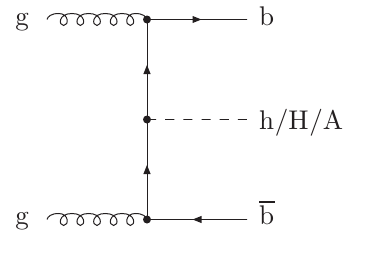
\includegraphics[height=3cm]{figure/bba.png}
            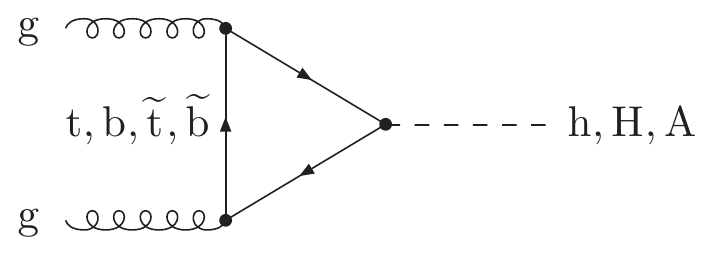
\includegraphics[height=3cm]{figure/ggf.png}

    \end{center}
    \caption{Feynman diagram for b-associated production and gluon-gluon fusion for MSSM neutral Higgs.}
   \label{fig:prod}
\end{figure}

\begin{figure}[tp]
     \begin{center}

            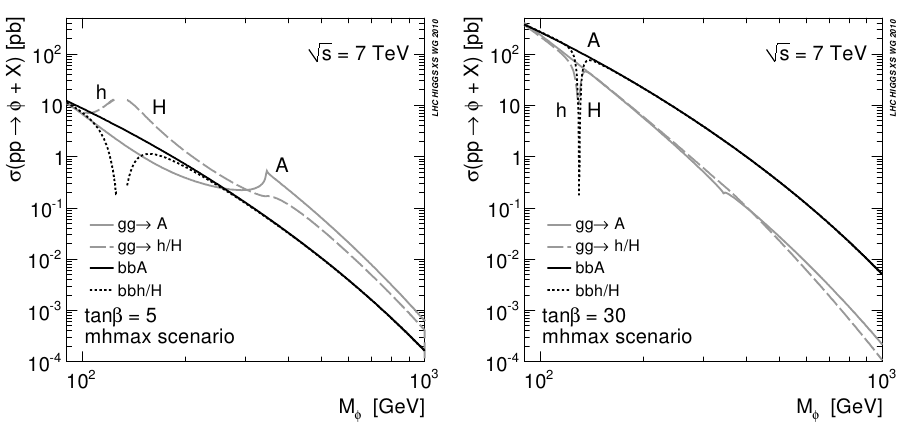
\includegraphics[width=\textwidth]{figure/xsec.png}

    \end{center}
    \caption{Production cross section for the \emph{h/H/A} MSSM neutral Higgs bosons via b-associated production and
	gluon-gluon fusion production mode. The calculation are for the $m_h^{max}$ scenario and for $\tan \beta=5$ (left) and $\tan \beta=30$ (right).}
   \label{fig:xsec}
\end{figure}

\begin{table}[t]
  \begin{center}
   \begin{footnotesize}	
    \begin{tabular}{cc}
      \hline \hline
      Channel & Selection \\
      \hline
      Preselection 	&  Trigger \\
	&	At least one reconstructed vertex \\
	&	Event cleaning	\\
	&	Tau Veto \\
	& 	Exactly one tight isolated electron with $\pt > 15 $ or 25 GeV (trigger dependent) \\
	&	Exactly one Combined isolated muon with  $\pt > 10$ GeV \\
	& 	Opposite charge between the leptons \\ 
      \hline
      b-Tag & Exactly one b-tagged taggable jet \\
      & $\Delta\phi(e-\mu)>2$ \\
      & $\sum\cos\Delta\phi > -0.2$ \\
      & $\sum H_T < 100$ GeV \\
      & $\SumLtMET < 100$ GeV \\
      & Good MMC solution \\
      \hline
      b-Veto & Exactly zero b-tagged taggable jets \\	
      & $\Delta\phi(e-\mu)>1.6$ \\
      & $\sum\cos\Delta\phi > -0.4$ \\
%      & $\SumLtMET < 150 \GeV$ \\
      & Good MMC solution \\
      \hline \hline
    \end{tabular}
    \caption{Summary of the preselection and the full selections used for the b-tag and b-veto channels.}
    \label{tab:sel}
  \end{footnotesize}
  \end{center}
\end{table}



The signal events considered in this search are  characterised by the presence of one electron, one muon and 
four neutrinos, the latter are associated to missing transverse energy of the event. Furthermore, 
additional b-tagged jets may be present if the the Higgs boson is produced in association with b-quark.
According to the signal events caractheristics, each event either data and MC should satisfy
the following selection criteria, these selections are shared by both analysis category and therefore 
referred in the following as ``common selections'':


\begin{enumerate}[label=(\roman*)]
\item Trigger requiring the presence of an electron with $\pt > 24$ GeV, or alternativaley,
	an electron with  $\pt > 12$ GeV togheter with a muon with  $\pt > 8$ GeV. 
	{\em \footnotesize  Note to Sandra: should I mention that the trigger is a selection during data taking?
	Or is the trigger is supposed common knowledge?}

\item Exactly one reconstructed electron and one muon of opposite charge should be present in the event. The muon is required to have $\pt > $ 10~GeV, while the electron 
should have $\pt > $ 15 or 25~GeV depending on the trigger that selected the event. For definition of reconstructed electron and muon object 
see chapter~\ref{chap:detector}.

\item The two leptons should be isolated, meaning that in a cone around the lepton there should be little energy deposit (should not be sorraunded by                 
other particle, common of non-promt leptons coming from jets). For more detail about isolation properties see section ~\ref{sec:BackgroundEstimation}.

\item The events is rejected if at least one jet from hadronic $\tau$ decay is found with $\pt > $ 15 GeV.

\item The invariant mass of the sum of the electron and muon 4-vectors should be greather than 30 GeV.
\end{enumerate}
This set of selection all togheter are referred in the following as \emph{preselection}. More detail on preselections 
are reported in table~\ref{tab:sel}, for details on object reconstruction and quality requirements see chapter~\ref{chapted:detector}. 
The two analysis category, \emph{b-tag} and \emph{b-veto}, are defined adding on top of the preselections 
the request of "exactly one b-tagged jet" or "no b-tagged jet" in the event respectively, to be 
\emph{taggable} a jet should have $\pt > 20$ GeV and $|\eta| < 2.5$.


\subsubsection{Event Category}\label{sec:selectiona}
%\subsection{Selections}

The final state of Higgs decaying into tau pair coincide with the one from  $\Ztautau$  process, this is then an irreducible 
background. Exploiting the different kinematics of the Higgs decay with respect to other backgrounds it possible to disentangle
between the two. In the Higgs decaying into $\tau^{+} \tau^{-} \rightarrow e ~ \mu + 4\nu$ the taus are highly boosted
and this feature is transferred to the final state leptons, their kinematics then result to be  significantly different 
with respect to process like diboson or $\ttbar$. A first difference is that  $e$ and $\mu$ from the Higgs decay will be more likely "back-to-back",
as it is shown in Figure~\ref{dphi} where the angle between the leptons in the transverse plane $\Delta\phi = |\phi_{e} - \phi_{\mu}|$ 
is reported.  Furthermore the neutrinos will be more likely collinear with the charged leptons:
this feature can be matematically seen as the sum of scalar product between missing energy and the leptons four-vectors in the
transverse plane, if the vectors are normalised to unit versors then what remains is a relation only between angles:
$$ \hat{E}_{T}^{miss} \cdot ( \hat{P}_{T}^{\mu} + \hat{P}_{T}^{e} ) = cos(\Delta\phi_{E_{T},\mu}) + cos(\Delta\phi_{E_{T},e}) = \sum_\ell cos(\Delta\phi_{E_{T},\ell}) $$
collinearity implies this sum to be equal to zero as it is shown in Figure~\ref{sumcosphi}. 
These two feature can be used to distinguish between mu-e coming from decay from highly 
boosted object and the one coming from W decays in top or in dibosons backgrounds which will have a more spread distribution.
In b-veto category these two variables are sufficient to suppress contribution from dibosons,
no other selection is applied in this category because it has been shown to not bring significant improvement.

In the b-tag category the situation is different, 
the  request of b-jet enhance backgrounds with high jet activity as top production, given the relatively low
jet activity of Higgs events (also in the case of b-associated production) it is possible to separate them from
top production which instead is very likely to have two or more highly enegetic jets in the event.
Little jet activity is achieved by requesting requesting the sum of the jets $\pt$ in the event to be small, this variable is called $\Ht$
and is shown in Figure~\ref{Ht}.
Another feature that distinguish top pair production from Higgs is the much higher invariant mass of the former final state,
in the transverse plane all the leptons will tend to have a higher momentum, the sum of lepton \pt and \met is then used as
a discriminating variable. Figure~\ref{sumlepPt} shows the distribution of this last analysis variable.

The above described variables defines the signal region in the b-tag and b-veto category,
in table~\ref{tab:sel} a summary of the preselection and all the selection variable used with their optimized cut values is reported.
Figure~\ref{fig:mass} shows the final state invariant mass distribution (here the \mmc 
discriminating variable is used see section~\ref{sec:mmc}) as a function of the selection stage,
while in tables~\ref{tab:eventsel:bveto}-\ref{tab:eventsel:btag} the number of events that survises at each cut stage for different background is reported.

\begin{figure}[p]
     \begin{center}
     \subfigure[]{		
            \includegraphics[page=11,width=0.47\textwidth]{figure/std_plots_presel.pdf}
	    \label{dphi}	
     }	
     \subfigure[]{		
            \includegraphics[page=12,width=0.47\textwidth]{figure/std_plots_presel.pdf}
	    \label{sumcosphi}	
     }	
     \subfigure[]{		
            \includegraphics[page=9,width=0.47\textwidth]{figure/std_plots_presel.pdf}
	    \label{Ht}	
     }	
     \subfigure[]{		
            \includegraphics[page=10,width=0.47\textwidth]{figure/std_plots_presel.pdf}
	    \label{sumlepPt}	
     }	

    \end{center}
    \caption{Distribution of analysis variable after preselection.}
   \label{fig:selections}
\end{figure}


\subsection{Mass Reconstruction with MMC Technique}\label{sec:mmc}

Acurate invariant mass reconstuction of a di-$\tau$ resonace is a challenging task
due to the presence of neutrinos from the $\tau$ leptons decay. 
In case of leptonic decay of both $\tau$ leptons a pair of neutrinos for each
of them are involved in the final state,  the system presents then eight uknowns, which corresponds to the four-momentum of the neutrinos pairs.
Four additional kinematic constraint are set by the following equations:
%There are four additional constraint 
%which come from the measurement of \MET and from the fact that each single decay should have invariant mass equal to the tau mass:
\begin{equation} \label{eq:MMC}
\begin{split}
%\begin{align}
%\begin{gather*}  
&\vec{E}_T^{miss} = \vec{P}_{T}^{mis_{1}} +  \vec{P}_{T}^{mis_2} \\
&M_{\tau_{i}}^2 = m^2_{mis_{i}} + m^2_{vis_{i}} + 2 \mathbf{P}_{vis_i} \cdot \mathbf{P}_{mis_i} \\
%\end{align}
%\end{gather*}
\end{split}
\end{equation}
where the index \emph{i} runs over the two $\tau$ leptons of the event and assumes the values of 1 or 2, 
$\vec{P}_{T}^{mis_{i}}$, $m_{mis_{i}}$ and $\mathbf{P}_{mis_{i}}$ are respectively the transverse momentum, the invariant mass and 
the four momentum of the pair of neutrinos related to the  $\tau$ lepton decay \emph{i} with mass $M_{\tau}$, the subscript \emph{vis} indicates insetad 
quantities related to the charged lepton from  $\tau$ lepton decay. The system has still four degrees of freedom,
%$m^2_{miss}$, therefore there are still four degrees of freedom in the system.
several approximation are possible to further constraint the momentum carried by neutrinos,
for example assuming them collinear to the electron or muon from $\tau$ lepton decay, however those approximation 
suffers of mass resolution limitations.

In this analysis, the so-called "Missing Mass Calculator" (MMC) algorithm
is used to calculate the most likely di-$\tau$ system invariant mass given the event topology, %event kinematics
the implementation of the method in this search is based on~\cite{MMC}. 
The concept of the MMC is to solve equation~\ref{eq:MMC} assigning values to the yet undetermined variables, performing a 
``scan'' over a four dimensional parameter space. The four independent  variables are chosen 
to be $ m^2_{mis_{i}}$ and $cos\theta^*_i$ , the latter defined
as the angle between the charged lepton from the $\tau$ lepton decay and the boost direction of the $\tau$ lepton. 
The di-$\tau$ invariant mass of the event can be calculated for each given point of the parameter space that solves equations~\ref{eq:MMC},
however, the solutions are not all equally likely and  the probability of a given $\tau$ decay configuration can be predicetd by means
of simulation (PYTHIA supplemented with TAUOLA package is used). Each point in the parameter space, corresponding
to a particular di-$\tau$ invariant mass, is then weighted by its probability to occur. 
The estimator for the final discriminant, the mass of the di-tau system \mmc, 
is the maximum of the weighted invariant mass distribution calculated for the scanned points.

The missing energy plays an important role in the MMC method and  its resolution has an impact on the calculation
of the invarian mass. To improve $\met$ resolution, a scan over a six dimensional parameter space is performed 
in a similar way as described above, in this case however, $\vec{E}_T^{miss}$ is also considered uknown and value are assigned 
to it according to its uncertainty. The probability of each solution is calculated and the final missing transverse
energy is given by the weighted mean of the scanned points. 

The final procedure consist in obtaining first an estimated for $\met$ by means of a six dimensional scan over the solution of equations~\ref{eq:MMC},
successively a four dimensional scan is performed fixing $\met$ to the updated value and calculating the most likely invariant mass 
of the di-$\tau$ system. Figure.....


 
%Accurate invariant mass reconstruction of a di-tau system is a challenging task due to the escaping neutrinos.
%In this analysis, with four neutrinos in the final state, the number of unknown largely exceed the number of constraints,
%several approximation are possible to further constraint the neutrinos, for example assuming them collinear to the 
%other leptons from tau decay, however those approximation suffers of limitations. 

%In this analysis we use the so called missing mass calculator (MMC)~\cite{MMC}
%technique for the calculation of the di-tau system invariant mass. This technique employs additional 
%information from the well known tau decay to constraint the system, this is achieved by minimising a likelihood function 
%defined in the kinematically allowed phase space region, the result is a more precise measurement of the di-tau 
%system invariant mass and a considerable improvement in resolution. The invariant mass distribution 
%calculated with the MMC technique is referred in the following as $\mmc$ and is used as discriminating 
%variable in the limits setting.

\begin{figure}[p]
     \begin{center}
     
     \subfigure[]{		
            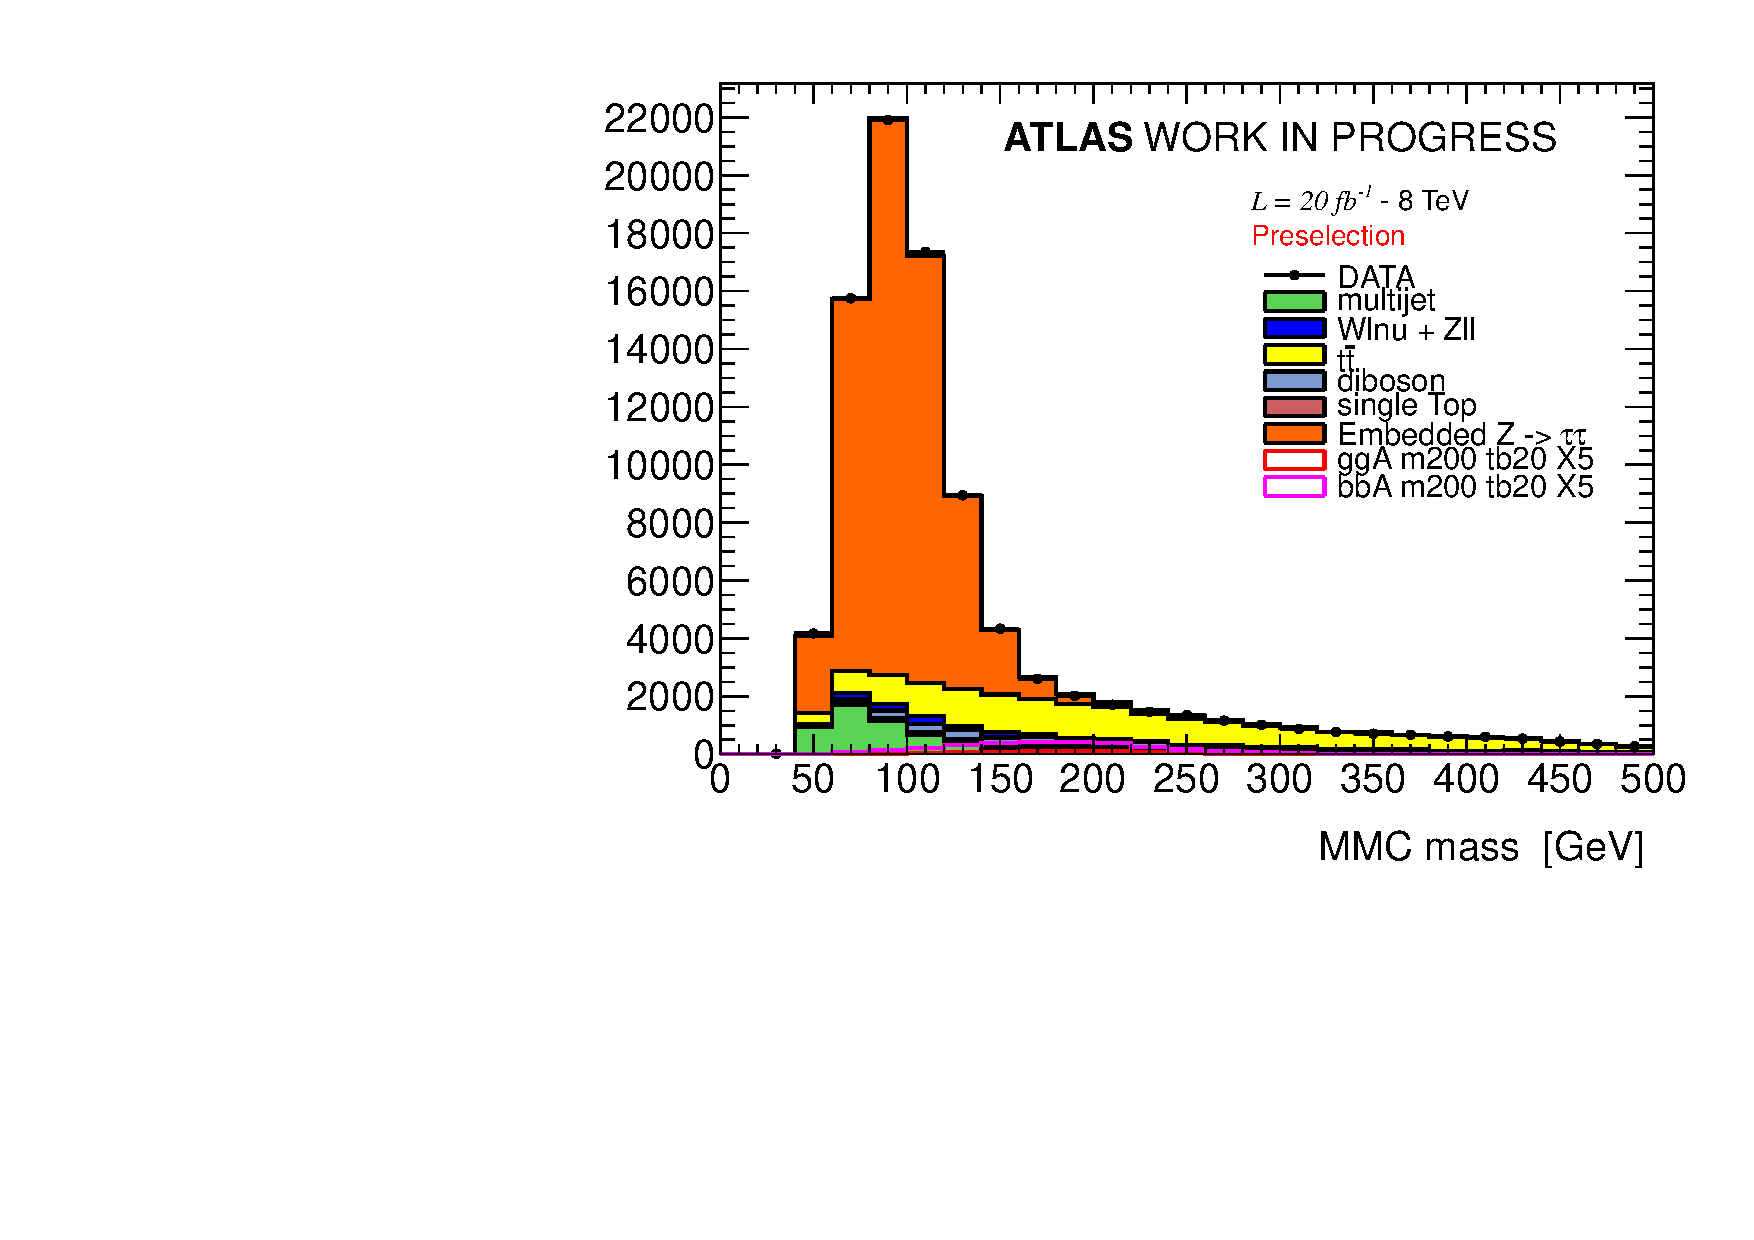
\includegraphics[page=1,width=0.47\textwidth]{figure/std_plots_mass.pdf}
	    \label{presel}	
    	%\caption{\footnotesize Preselection.}
     }\\	
    \end{center}

     \subfigure[]{		
            \includegraphics[page=3,width=0.47\textwidth]{figure/std_plots_mass.pdf}
	    \label{veto}	
    	%\caption{\footnotesize B-veto.}
     }	
     \subfigure[]{		
            \includegraphics[page=2,width=0.47\textwidth]{figure/std_plots_mass.pdf}
	    \label{tag}	
    	%\caption{\footnotesize B-tag.}
     }	
     \subfigure[]{		
            \includegraphics[page=5,width=0.47\textwidth]{figure/std_plots_mass.pdf}
	    \label{fullveto}	
    	%\caption{\footnotesize full B-veto.}
     }	
     \subfigure[]{		
            \includegraphics[page=7,width=0.47\textwidth]{figure/std_plots_mass.pdf}
	    \label{btagphi}	
    	%\caption{\footnotesize B-tag + $\Delta\phi$ + $\sum_\ell cos(\Delta\phi_{E_{T},\ell})$.}
     }
     
     \subfigure[]{		
            \includegraphics[page=6,width=0.47\textwidth]{figure/std_plots_mass.pdf}
	    \label{fullbtag}	
    	%\caption{\footnotesize full B-tag.}
     }
     	

    \caption{\footnotesize Distribution of the \mmc for different cuts stage, see text. Left column corresponds to b-tag category, right column to b-veto.}
   \label{fig:mass}
\end{figure}



\begin{sidewaystable}
  \centering
   \begin{footnotesize}	
  \begin{tabular}{ccccccccc}
    \hline\hline
	& Preselection			&	n(b-jet)=1			&	$\Delta\phi(e-\mu)>2$			&	$\sum\cos\Delta\phi > -0.2$			&	$\SumLtMET < 100 $ GeV			&	$\sum H_T < 100$ GeV			&	mmc			\\
   \hline
Data	&	125886			&	23352			&	-			&	-			&	-			&	-			&	-			\\
Multijet	&	6700	$\pm$	500	&	330	$\pm$	40	&	208	$\pm$	27	&	135	$\pm$	22	&	114	$\pm$	17	&	100	$\pm$	15	&	100	$\pm$	15	\\
\Zll 	&	570	$\pm$	50	&	5.2	$\pm$	1.8	&	2.3	$\pm$	1.1	&	2.3	$\pm$	1.1	&	1.7	$\pm$	1.0	&	0.9	$\pm$	0.8	&	0.9	$\pm$	0.8	\\
\Wlnu	&	1630	$\pm$	150	&	20	$\pm$	6	&	15	$\pm$	6	&	13	$\pm$	6	&	10	$\pm$	6	&	10	$\pm$	6	&	10	$\pm$	6	\\
Diboson	&	9340	$\pm$	50	&	99	$\pm$	5	&	63	$\pm$	4	&	36.4	$\pm$	3.0	&	14.8	$\pm$	1.8	&	13.3	$\pm$	1.8	&	13.1	$\pm$	1.8	\\
\ttbar	&	40630	$\pm$	110	&	19810	$\pm$	70	&	9680	$\pm$	50	&	6450	$\pm$	50	&	808	$\pm$	15	&	350	$\pm$	10	&	330	$\pm$	10	\\
Single Top	&	4450	$\pm$	40	&	2456	$\pm$	33	&	1223	$\pm$	23	&	784	$\pm$	18	&	122	$\pm$	7	&	99	$\pm$	7	&	90	$\pm$	6	\\
\Ztautau	&	61500	$\pm$	70	&	952	$\pm$	9	&	625	$\pm$	7	&	540	$\pm$	7	&	482	$\pm$	6	&	421	$\pm$	6	&	418	$\pm$	6	\\
Signal	&				&				&	-			&	-			&	-			&	-			&	-			\\
    \hline
    \hline
  \end{tabular}
  \caption{Number of data and background events in the b-tag channel.}
  \label{tab:eventsel:btag}
   \end{footnotesize}	
\end{sidewaystable}


%\begin{sidewaystable}
%  \centering
%  \begin{tabular}{ccccccccc}
%    \hline\hline
%   & Data & \Ztautau & \Zll &  \Wln & Single Top & \ttbar & Dibosons & Multi-jet \\
%   \hline
%Preselection & 188421	&79175.7 $\pm$	253.9	&853.4 $\pm$	66.6	&4977.5 $\pm$	387.3	&5265.5 $\pm$	48.9	&58575.1 $\pm$	175.7	&10726.5 $\pm$	51.3	&33831.6 $\pm$$\pm$	742.7 \\
%Exactly zero b-tagged jets & -	&78397.4 $\pm$	253.5	&840.3 $\pm$	66.2	&4905.7 $\pm$	386.8	&2235.2 $\pm$	34.3	&13313.3 $\pm$	93.9	        &10590.6 $\pm$	51.0	&31916.2 $\pm$	721.7 \\
%$\Delta\phi(e-\mu)>1.6$  & -	&75551.4 $\pm$	252.1	&725.2 $\pm$	62.7	&3503.7 $\pm$	307.8	&1492.3 $\pm$	27.9	&8465.6 $\pm$	73.1	        & 8387.3	$\pm$ 45.4 	&28831.1 $\pm$	594.7 \\
%$\sum\cos\Delta\phi > -0.4$ &-	&72161.7 $\pm$	249.8	&632.5 $\pm$	59.6	&2112.2 $\pm$	202.7	&925.1 $\pm$	22.5	&5635.9 $\pm$	59.0	        & 4535.9 $\pm$	33.3	        &23625.5 $\pm$	413.3 \\
%  \hline
%    \hline
%  \end{tabular}
%  \caption{Number of data and background events in the b-veto channel.}
%  \label{tab:eventsel:bveto}
%\end{sidewaystable}

\begin{table}
  \centering
   \begin{footnotesize}	
  \begin{tabular}{cccccc}
    \hline\hline
	&	Preselection			&	n(b-jet)=0			&	$\Delta\phi(e-\mu)>1.6$			&	$\sum\cos\Delta\phi > -0.4$ 			&	mmc			\\
    \hline
   \hline
Data	&	125886			&	89155			&	-			&	-			&	-			\\
Multijet	&	6693	$\pm$	456	&	6357	$\pm$	461	&	5322	$\pm$	438	&	4137	$\pm$	339	&	3934	$\pm$	335	\\
\Zll 	&	569	$\pm$	48	&	564	$\pm$	48	&	516	$\pm$	47	&	434	$\pm$	44	&	432	$\pm$	44	\\
\Wlnu	&	1625	$\pm$	155	&	1604	$\pm$	155	&	1145	$\pm$	125	&	714	$\pm$	101	&	656	$\pm$	100	\\
Diboson	&	9338	$\pm$	48	&	9235	$\pm$	48	&	7358	$\pm$	43	&	4002	$\pm$	31	&	2925	$\pm$	27	\\
\ttbar	&	40632	$\pm$	106	&	7707	$\pm$	46	&	5044	$\pm$	37	&	3416	$\pm$	31	&	2159	$\pm$	24	\\
Single Top	&	4449	$\pm$	44	&	1664	$\pm$	27	&	1124	$\pm$	22	&	682	$\pm$	18	&	435	$\pm$	14	\\
\Ztautau	&	61503	$\pm$	68	&	60440	$\pm$	67	&	58078	$\pm$	65	&	55303	$\pm$	64	&	54683	$\pm$	63	\\
Signal	&				&				&	-			&	-			&	-			\\
    \hline
  \end{tabular}
  \caption{Number of data and background events in the b-veto channel.}
  \label{tab:eventsel:bveto}
   \end{footnotesize}	
\end{table}
